\def\nubar{\ensuremath{\overline\nu}}
\def\nue{\ensuremath{\nu_e}}
\def\nuebar{\ensuremath{\overline{\nu}_e}}
\def\nutaubar{\ensuremath{\overline{\nu}_\{tau}}
\def\nuone{\ensuremath{\nu_1}}
\def\nutwo{\ensuremath{\nu_2}}
\def\nuthree{\ensuremath{\nu_3}}
\def\deltam{\ensuremath{\Delta m^2}}
\def\deltamthreeone{\ensuremath{\Delta m^2_{31}}}
\def\deltamtwothree{\ensuremath{\Delta m^2_{32}}}
\def\deltamonetwo{\ensuremath{\Delta m^2_{21}}}
\def\thetaonethree{\ensuremath{\theta_{13}}}
\def\sinthetaonethree{\ensuremath{sin \theta_{13}}}
\def\sintthetaonethree{\ensuremath{sin \theta_{13}^2}}
\def\sinsqtthetaonethree{\ensuremath{sin 2\theta_{13}^2}} 
\def\thetatwothree{\ensuremath{\theta_{23}}}
\def\sinthetatwothree{\ensuremath{sin \theta_{23}}}
\def\sintwothetatwothree{\ensuremath{sin \theta_{23}^2}}
\def\sinsqtwothetatwothree{\ensuremath{sin 2\theta_{23}^2}} 
\def\thetaonetwo{\ensuremath{\theta_{12}}}
\def\sinthetaonetwo{\ensuremath{sin \theta_{12}}}
\def\sintwothetatonetwo{\ensuremath{sin \theta_{12}^2}}
\def\sinsqtwothetaonetwo{\ensuremath{sin 2\theta_{12}^2}} 
\def\deltacp{\ensuremath{\delta_{CP}}}
\DeclareGraphicsRule{.tif}{png}{.png}{`convert #1 `dirname #1`/`basename #1 .tif`.png}

%\newcommand{\numu}{\ensuremath{\nu_{\mu}}}
%\newcommand{\numubar}{\ensuremath{\overline\nu_{\mu}}}
%\newcommand{\nutau}{\ensuremath{\nu_{\tau}}}
\newcommand{\mutoe}{\ensuremath{\nu_{\mu} \rightarrow \nu_e}}
\newcommand{\mubartoebar}{\ensuremath{\overline{\nu}_{\mu}\rightarrow\overline{\nu}_e}}
%\\newcommand{\hz}{\,\mathrm{Hz}}
%\newcommand\mutoe{\numu\rightarrow\nue}
%\\newcommand{\khz}{\,\mathrm{kHz}}
%\\newcommand{\mhz}{\,\mathrm{MHz}}
\newcommand{\ev}{\,\mathrm{eV}}
%\\newcommand{\kev}{\,\mathrm{keV}}
\newcommand{\mev}{\ensuremath{\,\mathrm{MeV}}}
%\\newcommand{\mevc}{\,\mathrm{MeV}/c}
%\\newcommand{\mevcc}{\,\mathrm{MeV}/c^2}
\newcommand{\gev}{\ensuremath{\,\mathrm{GeV}}}
\newcommand{\km}{\ensuremath{\,\mathrm{km}}}
\newcommand{\kw}{\ensuremath{\,\mathrm{kW}}}
\newcommand{\MW}{\ensuremath{\,\mathrm{MW}}}
\newcommand{\kt}{\ensuremath{\,\mathrm{kT}}}

%\\newcommand{\cmsq}{\,\mathrm{cm}^2}
%\\newcommand{\nm}{\,\mathrm{nm}}
%\\newcommand{\ms}{\,\mathrm{m}}
%\\newcommand{\msec}{\,\mathrm{ms}}
%\\newcommand{\nsec}{\,\mathrm{ns}}
%\\newcommand{\nux}{\nu_x}
%\\newcommand{\nuxbar}{\bar{\nu}_x}

%\\newcommand{\mutotau}{\numu\rightarrow\nutau}
%\\newcommand{\mutox}{\numu\rightarrow\nux}
%\\newcommand{\mubartoxbar}{\numubar\rightarrow\nuxbar}
%\\newcommand{\piplusdecay}{\pi^+ \rightarrow \mu^+ \numu}
%\\newcommand{\piminusdecay}{\pi^- \rightarrow \mu^- \numubar}
%\\newcommand{\pimue}{\pi \rightarrow \mu \rightarrow e}
%\\newcommand{\muplusdecay}{\mu^+ \rightarrow e^+ \nue \numubar}
%\\newcommand{\muminusdecay}{\mu^- \rightarrow e^- \nuebar \numu}
%\\newcommand{\sinsqtheta}{\sin^2 2 \theta~}
%\\newcommand{\pizero}{\pi^{0}}
%\\newcommand{\pip}{\pi^{+}}
%\\newcommand{\pim}{\pi^{-}}
%\\newcommand{\pipm}{\pi^{\pm}}
%\\newcommand{\Kp}{K^{+}}
%\\newcommand{\Km}{K^{-}}
%\\newcommand{\KL}{K^{0}_{L}}
%\\newcommand{\KS}{K^{0}_{S}}
%\\newcommand{\reaction}{\nuebar + p \to e^{+} + n\ \ \ ,}
%\\newcommand{\evsq}{{eV}^{2}}

\subsubsection{Introduction}

The purpose of the Long Baseline Neutrino Experiment is to measure all the neutrino oscillation parameters including the currently unknown values of the the CP violating  phase \deltacp\ and the neutrino mass hierarchy.  Matter effects compete with the 
CP violation effects, and the baseline needs to be optimized to be able to disentangle them. 

To detect these neutrino oscillations, a  broad-band neutrino beam  of
mean energy 3.5\gev\ is proposed to originate at FNAL and to be
directed underground 1300\km\ away to the Sanford Underground Research
Facility in South Dakota.  The advantage of the long baseline and
correspondingly high neutrino energy at maximal mixing is apparent in
Fig.~\ref{fig_lbne}, analogous to those shown for T2K and \NOvA. 

%\vspace{1.5cm}
\begin{figure}[hbp]\begin{center}
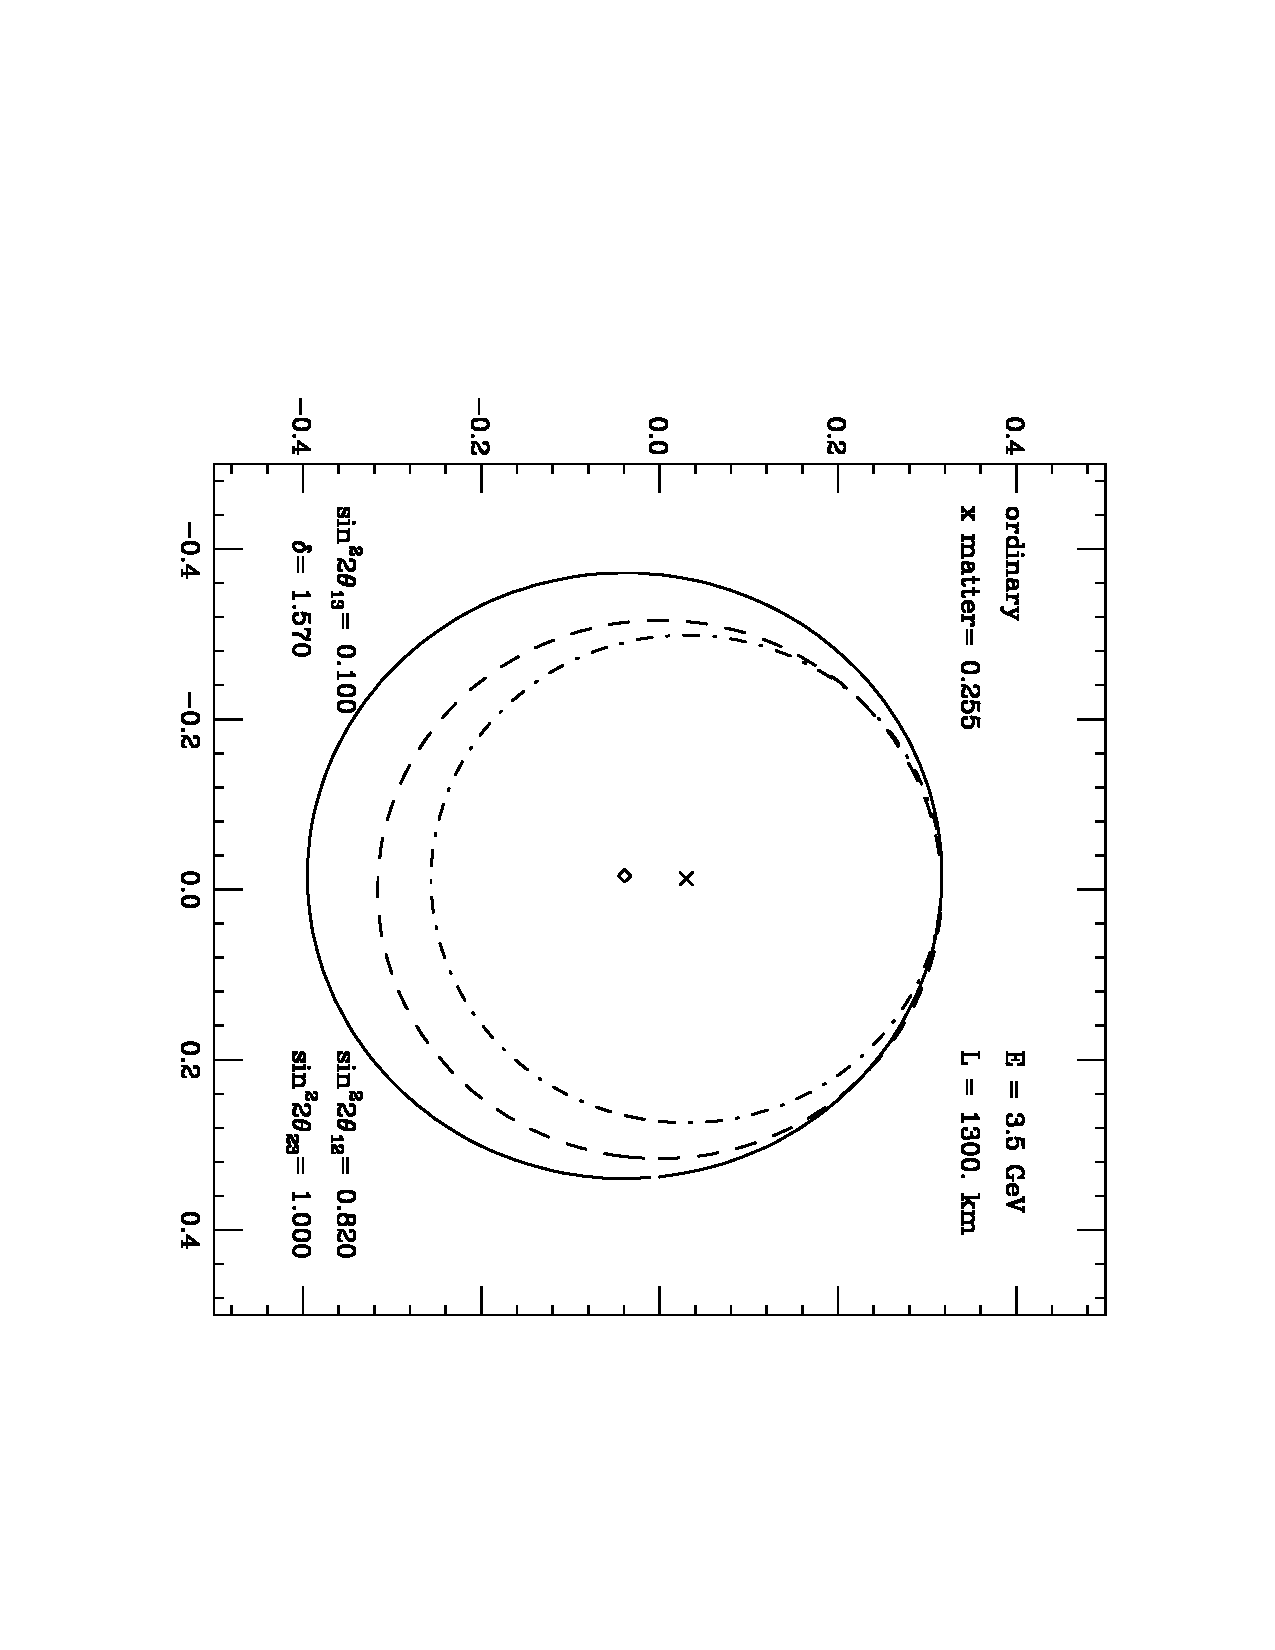
\includegraphics[width=2.5in,angle=90]{RNC/cpv_lbne_pibytwo.pdf}
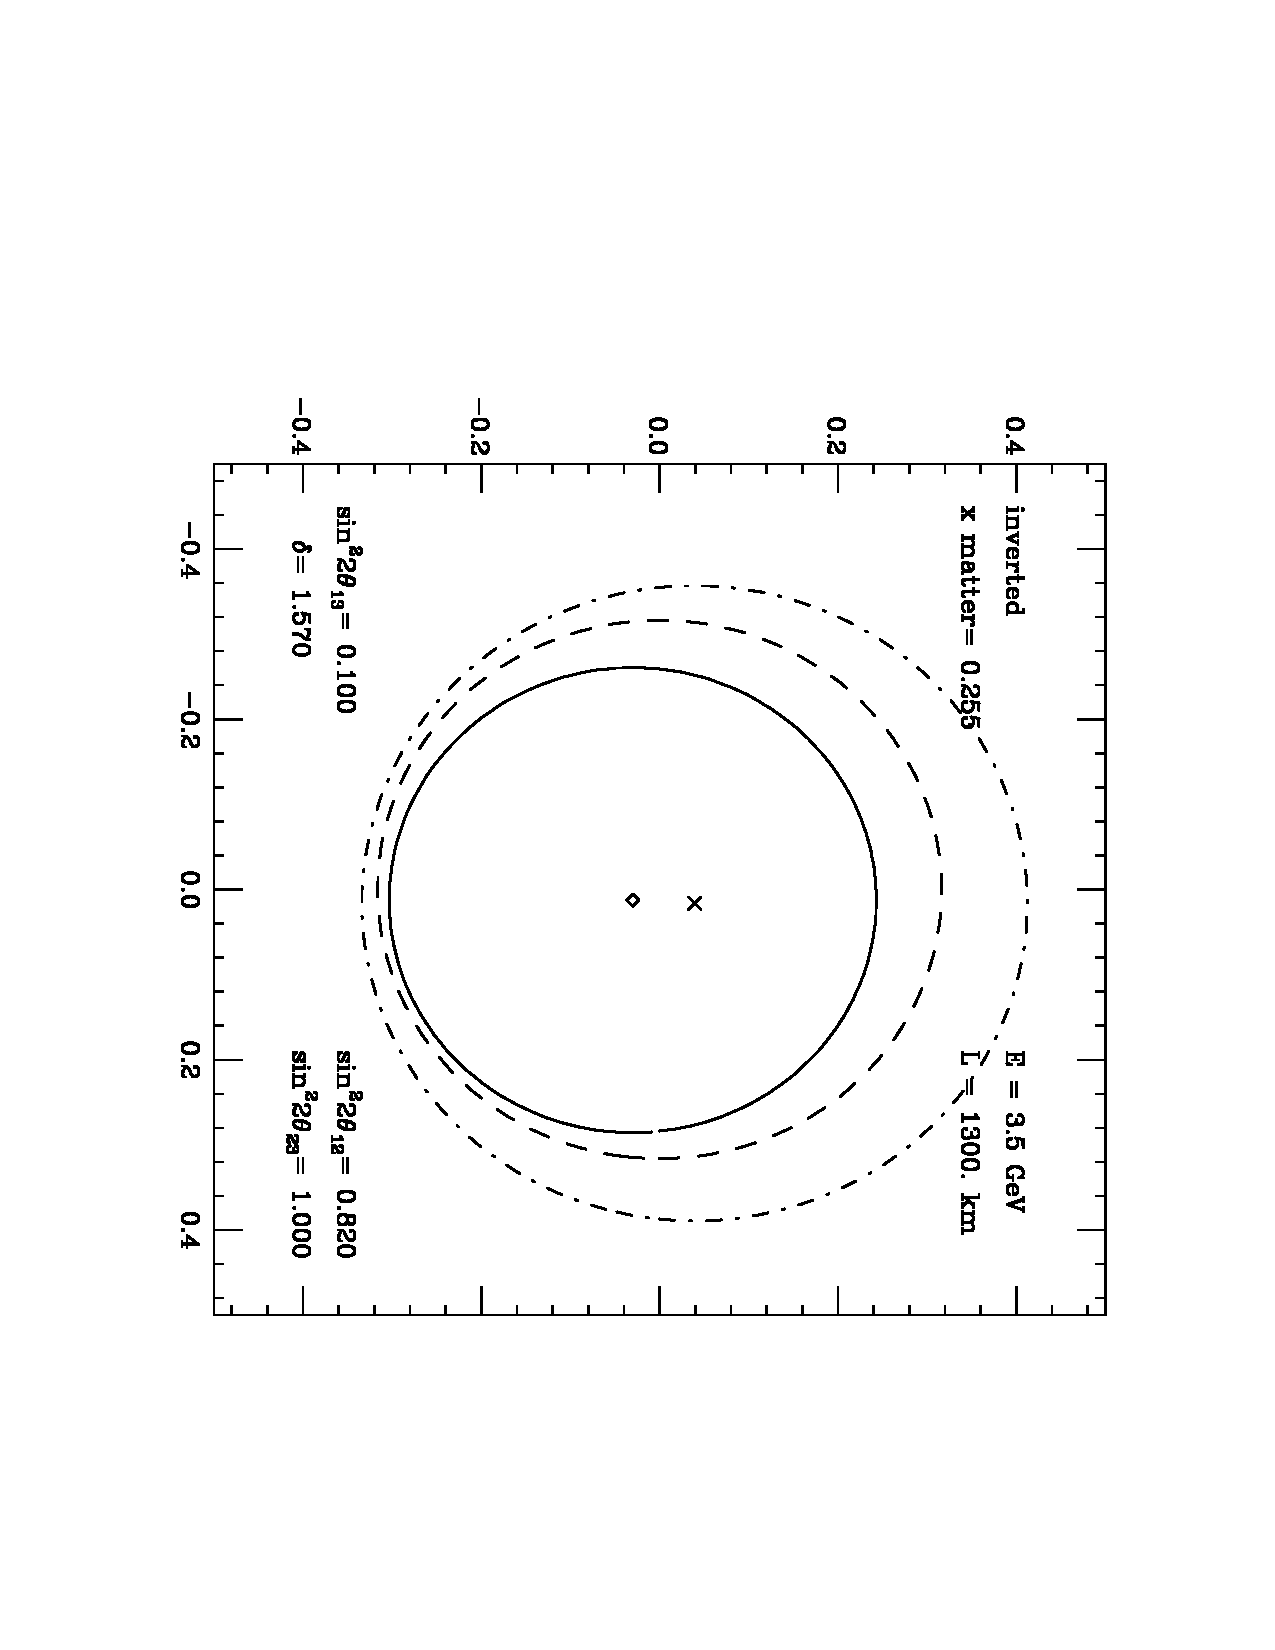
\includegraphics[width=2.5in,angle=90]{RNC/cpv_lbne_pibytwo_inv.pdf}
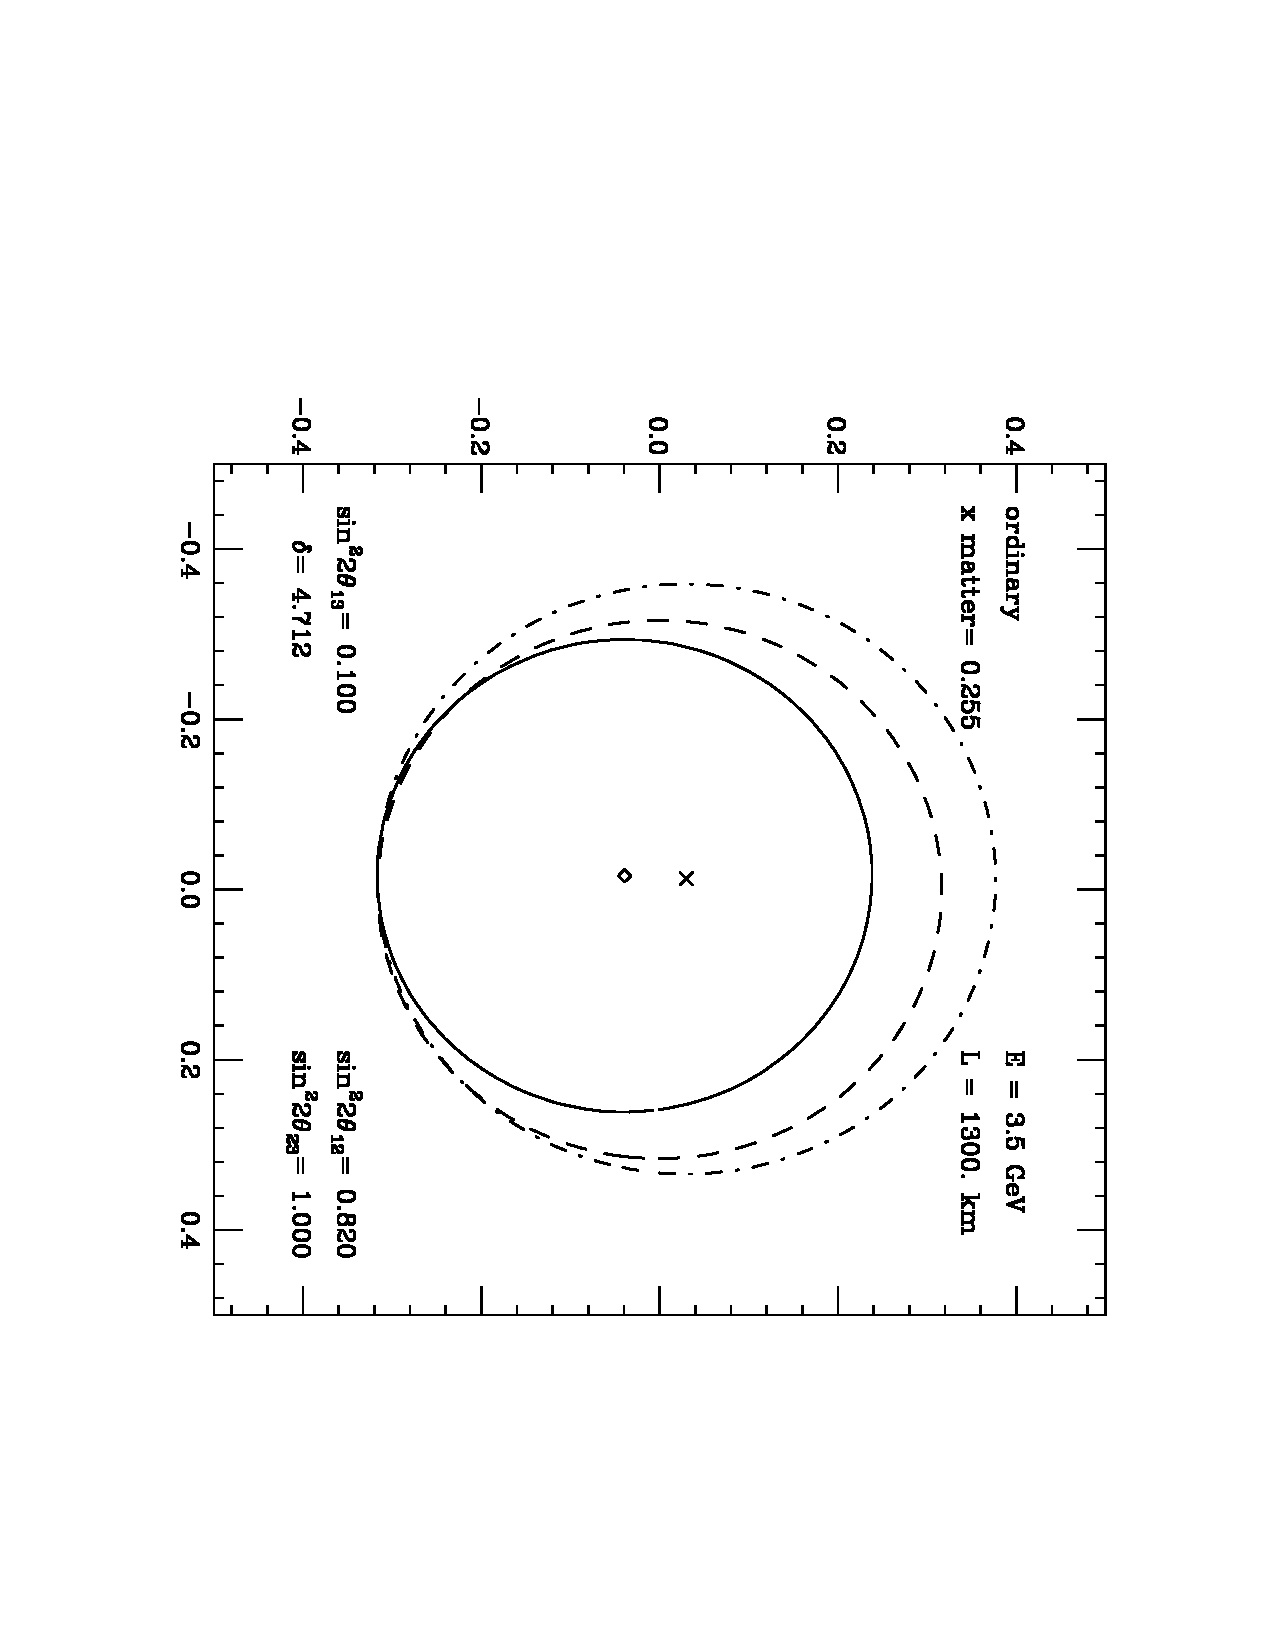
\includegraphics[width=2.5in,angle=90]{RNC/cpv_lbne_threepibytwo.pdf}
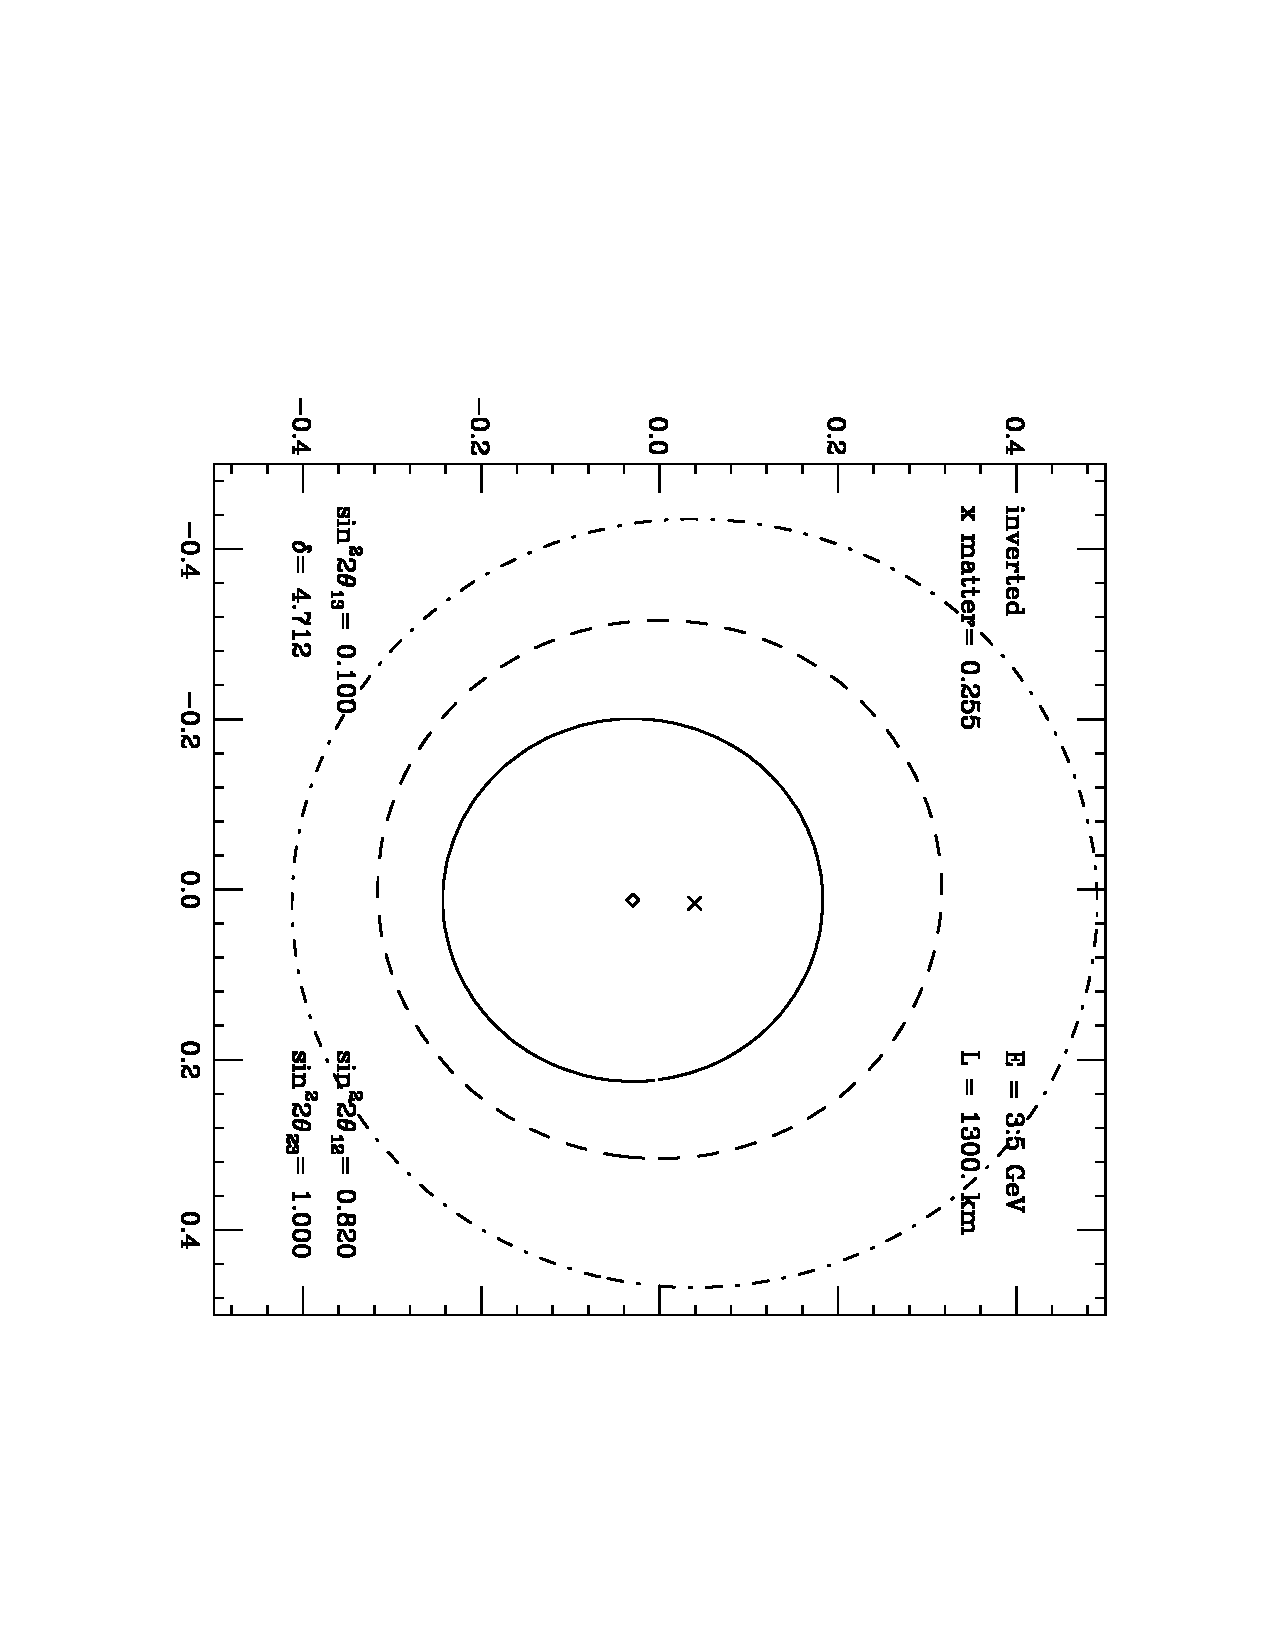
\includegraphics[width=2.5in,angle=90]{RNC/cpv_lbne_threepibytwo_inv.pdf}
\caption{Illustrative plots for a LBNE.  Upper, with true hierarchy
being normal, 
with $\deltacp=\pi/2$.  Lower, again with true hierarchy being normal,
but now with $\deltacp=3\pi/2$. The dot-dash circles show the
constraints from $\nu_\mu$ scattering, while the solid circles are for
$\nubar_\mu$.  The dashed circles show the constraints from a
hypothetical perfect measurement of $\sin^22\theta_{13}$.  The power
of LBNE is enhanced by combining with results from T2K (and to lesser
extent \NOvA) because the ``wrong'' solution occurs at different values
of $\deltacp$ for the three experiments. Note that the circles
correspond to a fixed beam energy of $3.5$~GeV, whereas the planned
neutrino beam is broadband. \label{fig_lbne}} 
\end{center}\end{figure}

%\clearpage
To maximize the event rate, the beam is typically tuned so that the
peak of the neutrino energy is at the first oscillation maximum for a
given distance, see Fig.~\ref{fig:BeamProfileNHandIH}. This is a
broad-band beam, optimized to cover both the first and second oscillation
maxima. Narrow band beams pick out a single energy and typically do
not sample the full distribution, but only a single  energy bin.  A
broad-band beam allows a measurement of the shape of the spectra
(including multiple maxima) favorable for the measurement
of \deltacp\, while a narrow band beam  only allows a counting
experiment at a single energy.  



\begin{figure}[tp]
\begin{center}
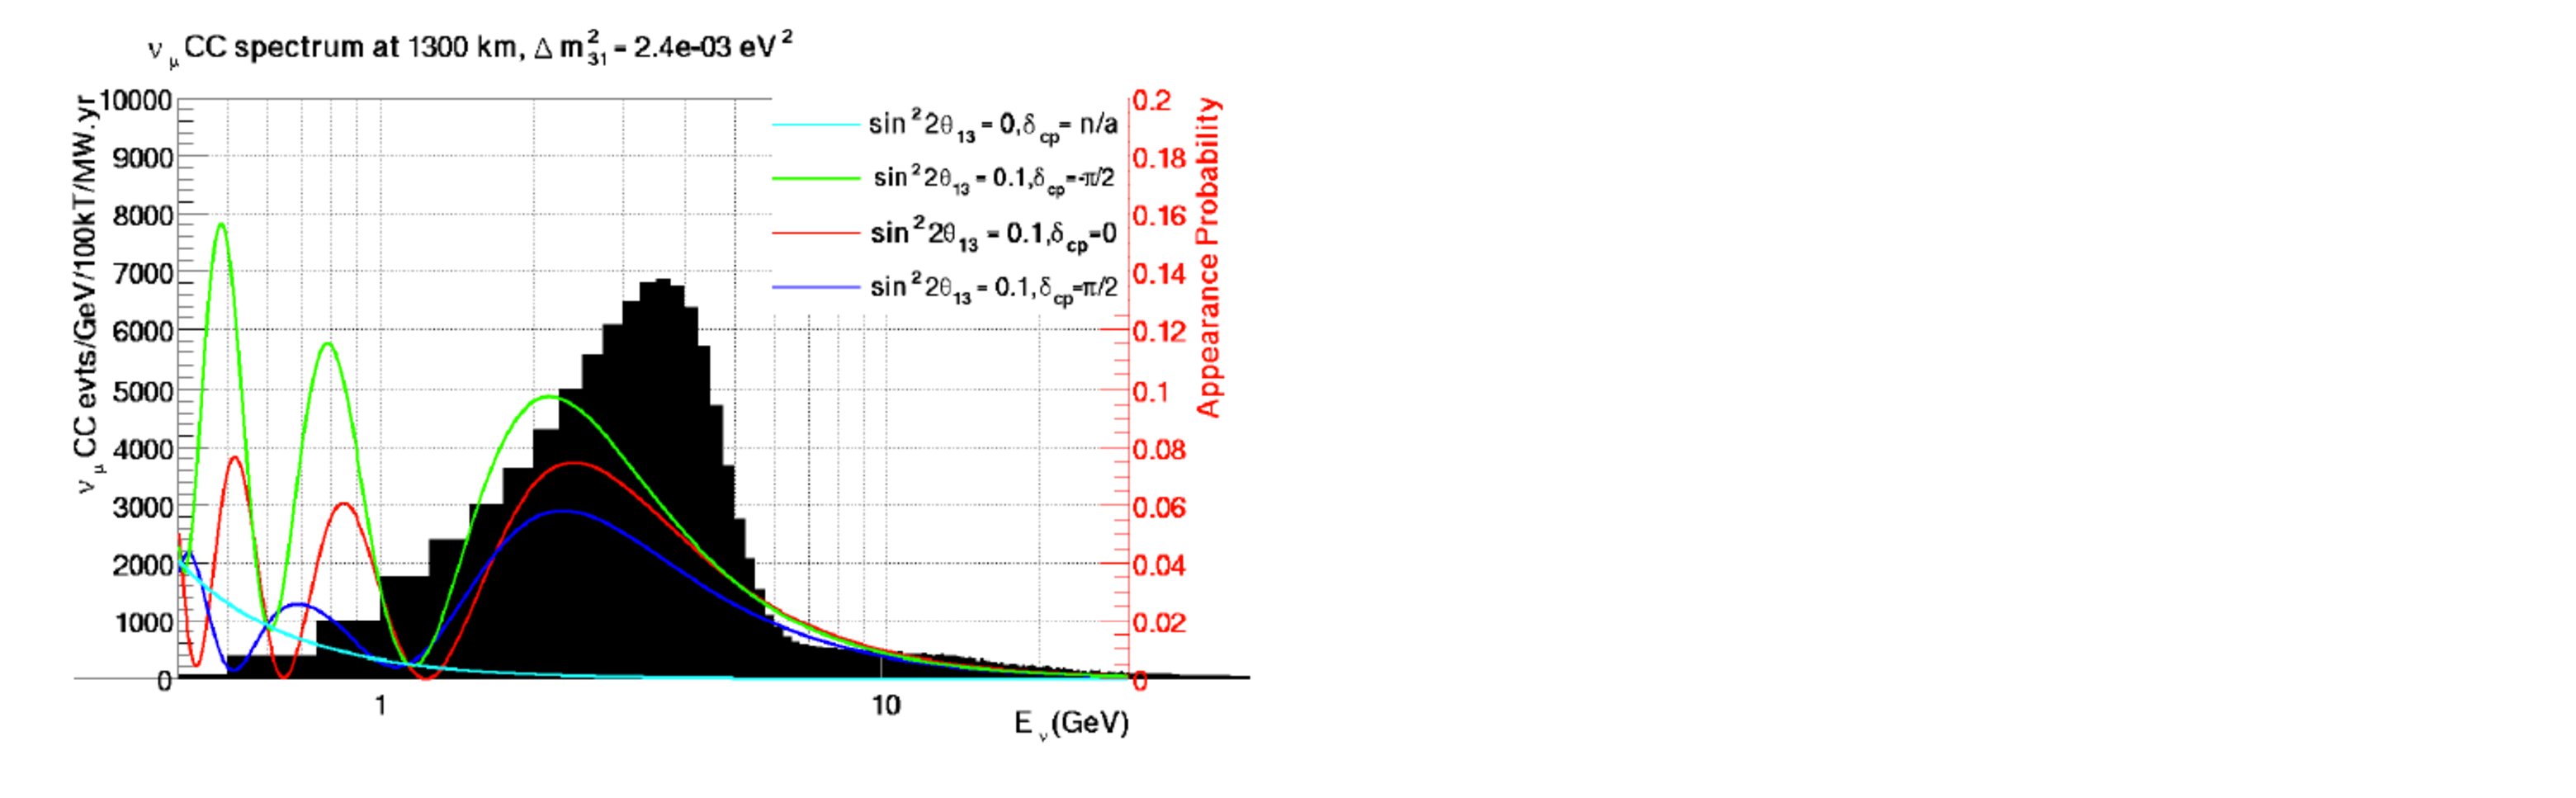
\includegraphics[width=0.7\textwidth]{RWK/LBNE/makefig1.pdf}
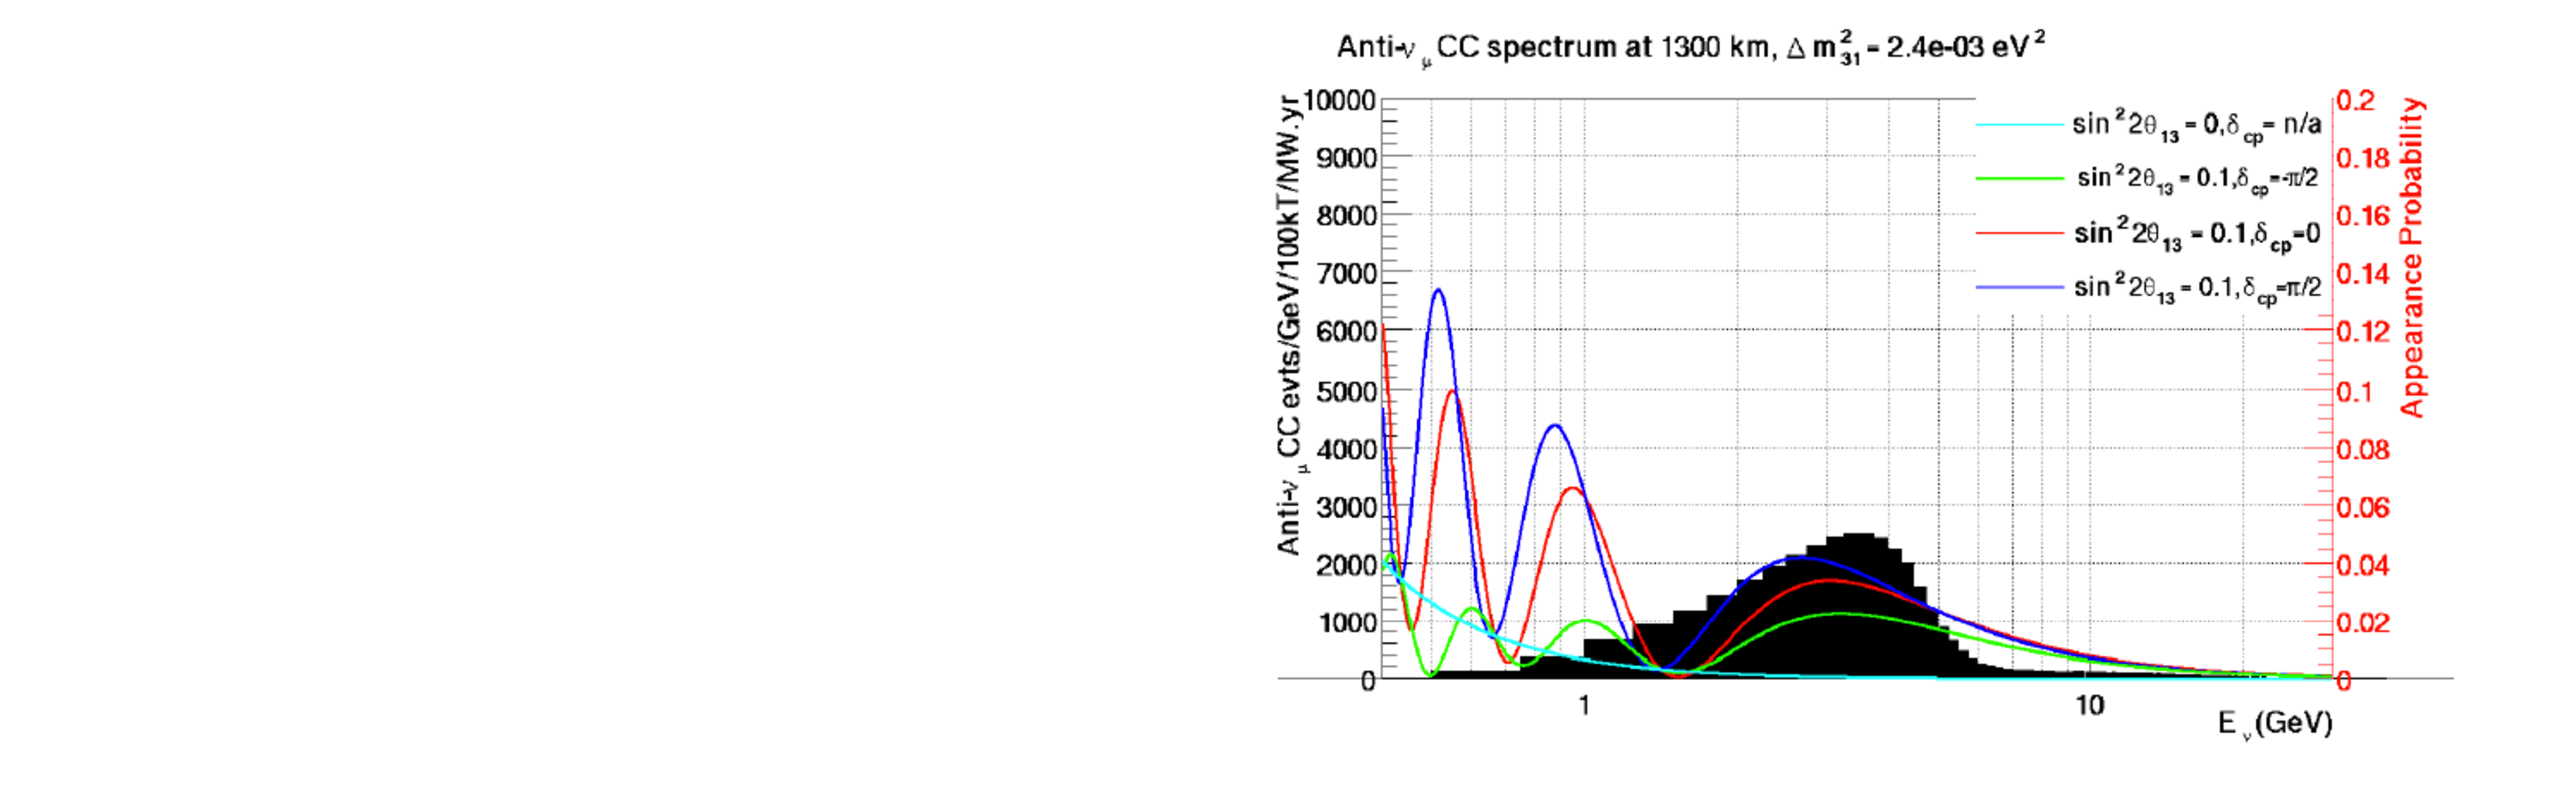
\includegraphics[width=0.7\textwidth]{RWK/LBNE/makefig2.pdf}
%\vspace{-0.8cm}
\caption{The black shaded areas are the unoscillated charged current spectra for the Homestake site (left-hand y-axis scale) at 1300 \km\ for \mutoe\ (top) and \mubartoebar\ transitions (bottom).  The colored lines are oscillation probabilities for different oscillation parameters, as given in the legend (right-hand y-axis scale). The maxima of the beam energy has been optimized to correspond to the  maximum of the first ``node,''  { \it{i.e.}} maximum of the probability of \mutoe\ transitions \cite{PWGReconfigurationReport}.}
\label{fig:BeamProfileNHandIH}
\end{center}
\end{figure}



\subsubsection{Phasing the Long Baseline Neutrino Experiment}

Due to budgetary constraints, the experiment is to be phased. 
The stated goal of the first stage of LBNE, as summarized in the recent HEPAP Major Facilities report, is to determine the hierarchy to greater than $3 \sigma$ for all values of the CP phase $\delta_{CP}$ (when constraints from other experiments are included), and to set the stage for a world-class US neutrino program that will include Project X, and physics goals such as a comprehensive search for CP violation.

The Phase I experiment consists of the beamline and a 10~kT liquid argon (LAr)
detector 
located on the surface at the SURF facility. The beamline at FNAL
includes a target, horn and decay tunnels consistent with accepting a
2.3\MW\ beam, and a set of instruments (an array of high pressure gas
muon Cherenkov counters, four layers of stopped muon detectors, and
two or three layers of hadron ionization detectors) at the absorber
complex to measure the flux, angle and centerline of the beam. There
is no near neutrino detector in the first phase.  The final phase
includes a 34~kT liquid argon detector, underground at the far site
and a substantial near detector most likely with  both a liquid argon
detector and a magnetized, high pressure Ar  [straw] tracker, and EM
calorimeter to measure the absolute neutrino flux via
neutrino-electron scattering. 

\subsubsection{Detector Performance}

The detector performance is evaluated in the context of the ``GLoBES''
software package~\cite{GLoBES}, which includes the energy spectrum of
the beam, interaction cross sections, the corresponding detector
efficiencies as well as specific  backgrounds and uncertainties {\it
{e.g.}} $\nutau$  backgrounds have recently been added, see
below. Table~\ref{fig:LArDetectorEfficiency} summarizes the properties
of the detector as coded into GLoBES. 

\begin{table}[!bp]
\caption{Estimated range of the LAr-TPC detector performance parameters for the primary oscillation physics. The expected
range of signal efficiencies, background levels, and resolutions from various studies (middle column) and the value chosen for
the baseline LBNE neutrino-oscillation sensitivity calculations (right column) are shown. For atmospheric neutrinos this is
the misidentification rate for events below 2 GeV; the misidentification rate is taken to be zero events  above 2 GeV \cite{PWGReconfigurationReport}.}\begin{center}
%\vspace{-0.6cm}
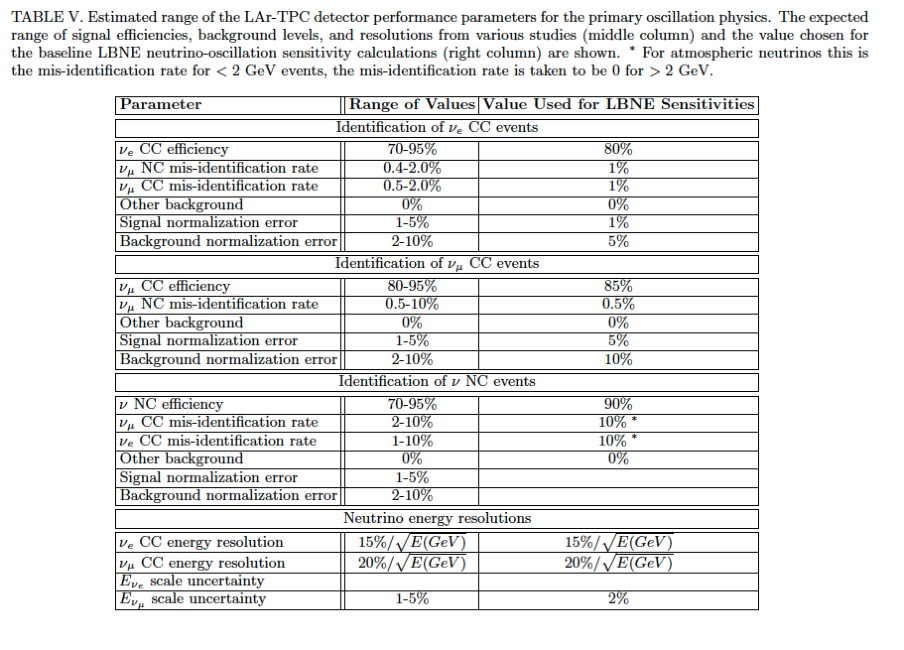
\includegraphics[trim = 0cm 0cm 0cm 2cm, clip=true, width=1.0\textwidth]{RWK/LBNE/LArDetctorEffeciencyTable.pdf}
\label{fig:LArDetectorEfficiency}
\end{center}
\vspace{-1.2cm}
\end{table}


Fig.~\ref{fig:SMMH} shows the range of sensitivity to the hierarchy for LBNE Phase I, both alone and in combination with T2K+NO$\nu$A.  
The left panel of Fig.~\ref{fig:MHsensitivityVsSize} shows the $2\sigma$ and $3\sigma$ sensitivity limits on the hierarchy as a function of  detector mass at the SURF site, and the right panel shows the 3$\sigma$ and 5$\sigma$ sensitivities to \deltacp.  

\begin{figure}[htbp]
\begin{center}
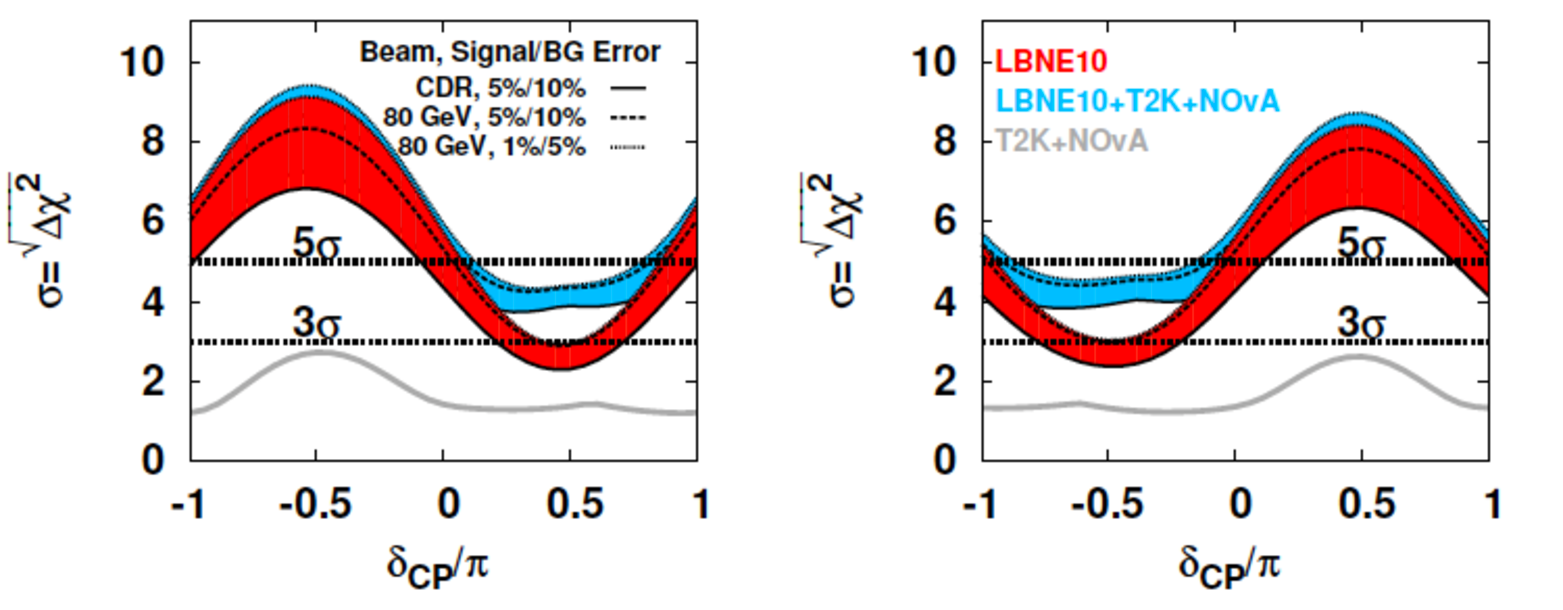
\includegraphics[width=0.9\textwidth]{RWK/LBNE/SMMH.pdf}
\caption{Mass hierarchy sensitivity for Phase I of LBNE alone (red band) and in combination with T2K+NO$\nu$A (blue band) for (Left) normal and (Right) inverted mass hierarchies~\cite{lbne:sm}.}
\label{fig:SMMH}
\end{center}
\end{figure}

\begin{figure}[htbp]
\begin{center}
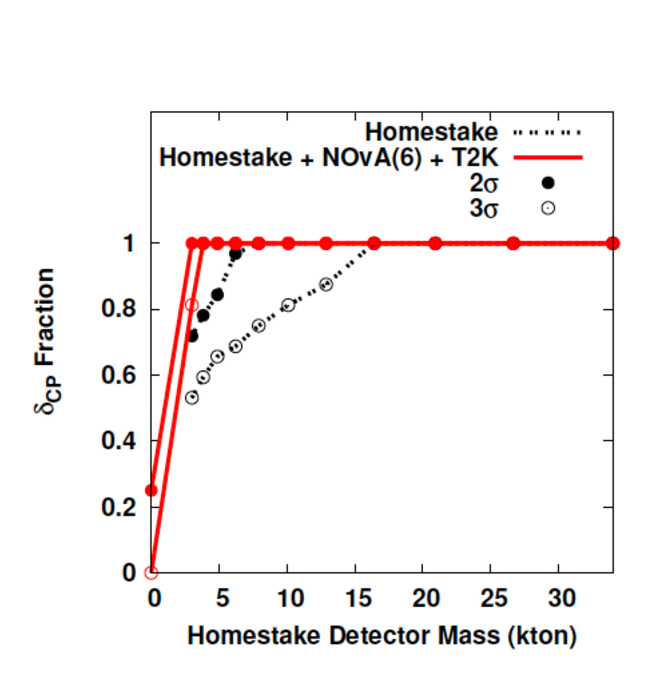
\includegraphics[width=0.5\textwidth]{RWK/LBNE/TwoAndThreeSigMHSentivityVsLArMass2.pdf}
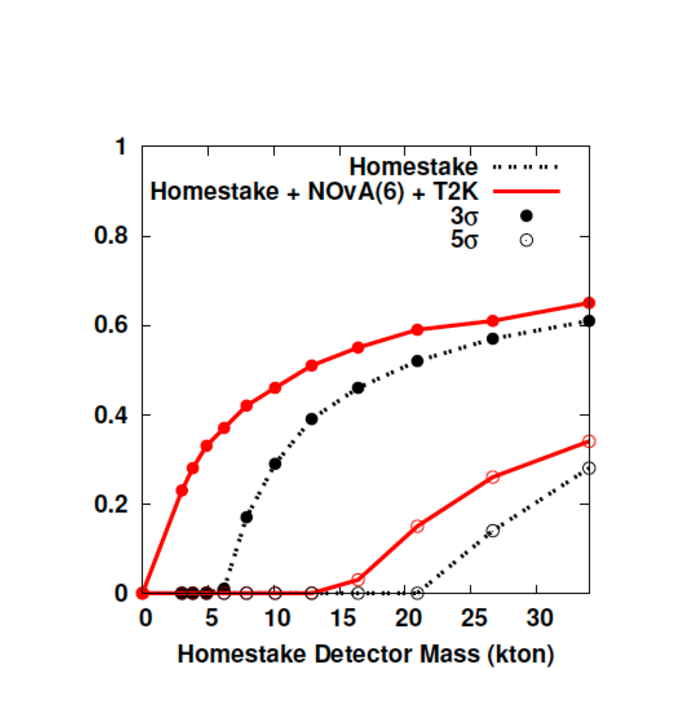
\includegraphics[width=0.45\textwidth]{RWK/LBNE/CPCoverageFractionVsMassSURF22.pdf}
\caption{(Left) 2- and 3-$\sigma$ sensitivity to the mass hierarchy versus the fraction of  \deltacp\ coverage  and detector mass when located at SURF, under the assumption of a normal hierarchy. Solid points are  2$\sigma$ limits, while open circles are 3$\sigma$ limits. Black is for LBNE alone, with $5\nu+5\bar{\nu} $ years at 700 kW, and red is combined with results from \Nova\ and T2K. \cite{PWGReconfigurationReport}. \\ (Right) 3- and 5-$\sigma$ sensitivity to $\delta_{CP}$ versus the fraction of the CP phase \deltacp\ as a function of the mass of the detector at the SURF site, under the assumption of a normal hierarchy. Solid points are  3$\sigma$ limits, while open circles are 5$\sigma$ limits. Black is for LBNE alone, with $5\nu+5\bar{\nu} $ years at 700 kW, and red is combined with results from \Nova\ and T2K. \cite{PWGReconfigurationReport}.}
\label{fig:MHsensitivityVsSize}
\end{center}
\end{figure}



The value of \deltamtwothree\ is one of the limiting factors in the
ability of second generation reactor experiments to measure the mass
hierarchy. 
As a further example of the
capabilities of the experiment, 
LBNE will have an unprecedented capability to
measure \deltamtwothree. 
The precision with which \deltamthreeone\
$\sim$ \deltamtwothree\ can be measured is shown in
Fig.~\ref{fig:DeltaM31sqMeasumentError}, approaching $10^{-5}\ev^2$ for
a 10 year exposure of a 34\kt\ detector. 


\clearpage


\begin{figure}[htbp]
\begin{center}
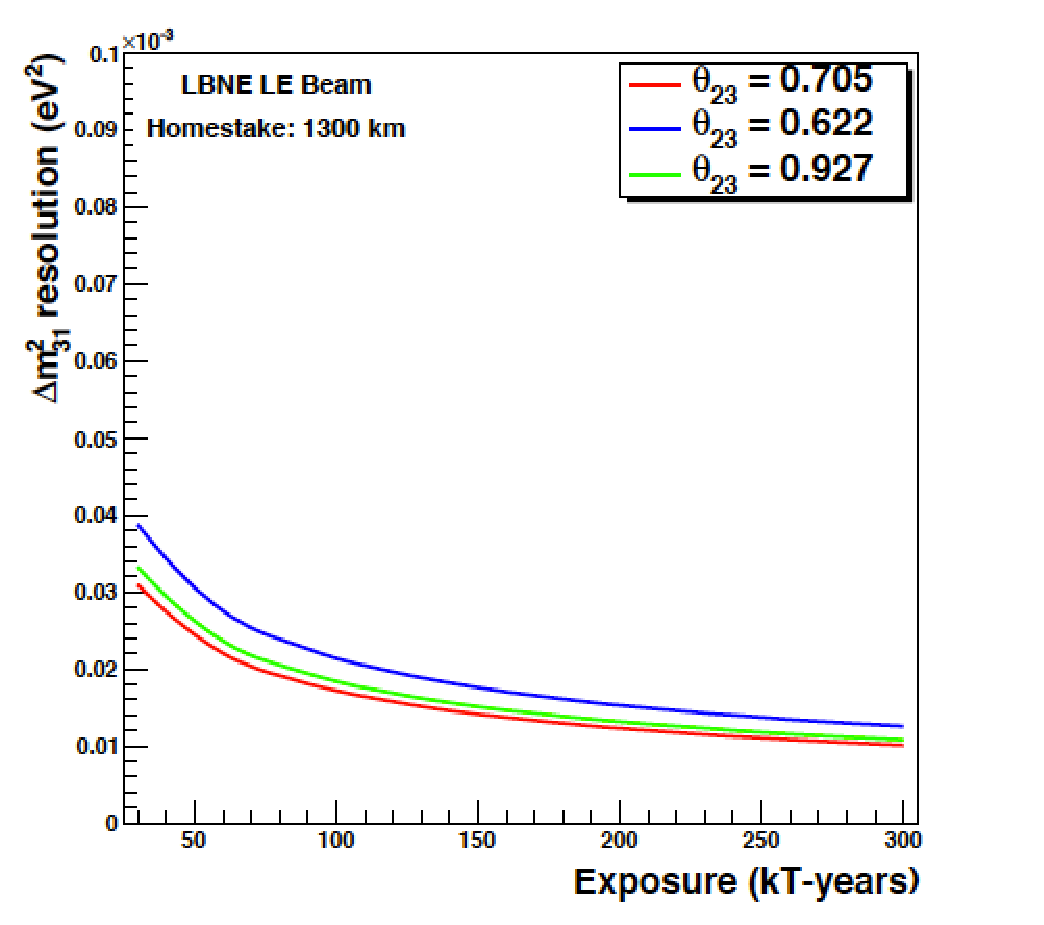
\includegraphics[width=0.7\textwidth]{RWK/LBNE/DeltaM31sqMeasumentError.pdf}

\caption{ Estimated error in \deltamthreeone\ $\sim$ \deltamtwothree\ versus detector exposure at 1300 km for three values of $\sin^2 2\thetatwothree$ [indicated in the legend only as \thetatwothree], for a 700\kw\ beam. 
Note the vertical scale (\deltamtwothree\  resolution) has a scale factor of $10^{-3}$.
The plot assumes a near detector for these precision measurements. Neutrino and anti-neutrino running are combined in the ratio of 1:1, The mass hierarchy is assumed to be known \cite{PWGReconfigurationReport}.}
\label{fig:DeltaM31sqMeasumentError}
\end{center}
\end{figure}




\subsubsection{Open Concerns}

There are four major concerns for the Phase I LBNE detector program:
\begin{enumerate}
\item {The surface location of the LAr detector;}
\item{The lack of a near detector;}
\item{The small mass (10\kt) of  the far detector;}
\item{Uncertainties in nuclear effects.}
\end{enumerate}

With a 10$\mu\mathrm{sec}$ beam window, the detector is live for approximately 100\,sec/year and assuming an overburden of 3m of rock the background from cosmogenically induced events is negligible,  less than $1\%$ in the \nue\ appearance experiment. Measuring \deltacp\ and the mass hierarchy can be accomplished by a LAr detector on the surface. Monte Carlo studies have shown that these measurements are statistics limited, and a simplified set of flux monitors at the end of the decay pipe at FNAL are sufficient to monitor the beam intensity.
For longer exposures (above 100 \kt\ $\times$ years), a near detector is needed, and collaborators from India have expressed interest in building such a detector.

A larger detector is attractive, and an excellent opportunity for
foreign investment. Some potential foreign collaborators have also
expressed interest in technical components of the beamline that would
help offset portions of the total project cost, and free DOE funds to increase
the scope of the US project. A smaller detector can also be offset via
higher beam intensity, and current plans at FNAL call for Phase I of
Project X to be completed by the start of LBNE, boosting the beam
power from 700\kw\ to $\sim1.1\MW$. This would effectively remove all
ambiguity in the 3$\sigma$ mass hierarchy measurement for all values
of \deltacp\  for a 10 year run of a 10kT LBNE LAr detector. 

Putting the detector underground would permit a broader physics
program, including proton decay searches and the detection of
neutrinos from supernova events. As a LAr
detector can easily  
identify charged kaons (which are below threshold in a water Cherenkov
detector), its sensitivity to proton decay quickly exceeds that of
SuperK by an order 
of magnitude summed over all decay modes, despite SuperK's
extrapolated 30yr integrated running history.   


The CD1 approval letter states that  LBNE may increase the scope of the project if additional resources can be found.
It is important to recognize that unlike other DOE/HEP projects where
the total project cost  (TPC) is usually capped, {\it including both
non-DOE domestic or foreign contributions, }in the LBNE case the
project has been given a ``hunting license'' to seek outside funding
to increase the {\it scope }of the project. Such negotiations are
ongoing.  

Construction of an unprecedentedly massive liquid-argon detector
presents significant technological challenges.  
It will require a  rigorous R\&D effort before the technology
is mature enough for this endeavor. 
If cost is not an issue, one approach in realizing this scheme is to modulize
the detector so that it can be staged. 

Nuclear effects will smear the reconstruction of the incident neutrino
energy \cite{Mosel}. A LAr detector is a ``tracking detector'' and
this may help in identifying low energy protons or gammas ejected from
the nucleus, but properly identifying neutrons may be problematic,
and extracting elementary reaction amplitudes for meson production is
difficult. The issue of the energy reconstruction in the presence of
these effects needs to be addressed.

